\documentclass{beamer} 
\usetheme{default} 
\usecolortheme{albatross}
\setbeamercovered{transparent}
%\useoutertheme{umbcfootline}  


\usepackage[spanish]{babel}
%\usepackage[latin1]{inputenc}
\usepackage[utf8x]{inputenc}
\usepackage{hyperref}
\usepackage{color}



\usepackage{multicol}



\title{String, Char y StringBuilder}

\author{Manuel J. Molino Milla \and Luis Molina Garzón}

\date{\today} %

\institute{IES Virgen del Carmen \and Departamento de Informática}





%\beamerdefaultoverlayspecification{<+->}

\begin{document}


\begin{frame}
  \titlepage
\end{frame}

\begin{frame}
    \frametitle{Logo}
\begin{figure}

\includegraphics[scale=1]{imagenes/logo.jpeg} 
\caption{Logo Java}
\end{figure}
\end{frame}

\begin{frame}
  \frametitle{Contenido}
  \tableofcontents[pausesections]
\end{frame}



\section{Clase String}


\begin{frame}
\frametitle{La clase String}
\begin{itemize}[<+->]
\item Un String es una secuencia de caracteres.
\item En Java, un String es un objeto.
\item Podemos crear un String:
\begin{enumerate}
\item String mensaje = new String(''Bienvenido a Java'');
\item String mensaje = ''Bienvenido a Java'';
\item char[ ] charArray = \{'G', 'o', 'o', 'd', ' ', 'D', 'a', 'y'\};
\end{enumerate}
\end{itemize}
\end{frame}

\begin{frame}
\frametitle{String en pila y montículo}
\framesubtitle{Gestión de referencias}
\begin{figure}
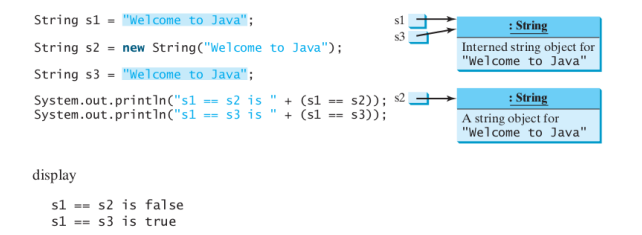
\includegraphics[scale=0.6]{imagenes/referencia.png}
\caption{Objetos String}
\end{figure}
\end{frame}



\begin{frame}
\frametitle{Clase String} 
\begin{multicols}{2}
\begin{figure}
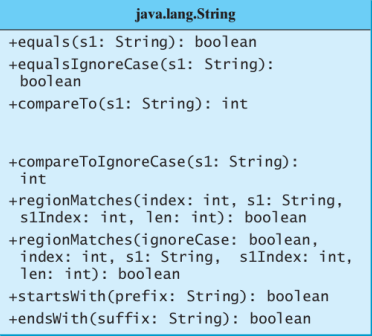
\includegraphics[scale=0.55]{imagenes/string.png} 
\caption{UML de la clase String}
\end{figure} 
\begin{scriptsize}
\begin{enumerate}[<+-| alert@+>]
      \item Devuelve true si el  string es igual al string s1.
      \item Devuelve true si el string es igual al string s1 \emph{case
insensitive}.
      \item Devuelve un entero mayor que 0, igual a 0, or menos que 0 para indicar si el string es mayor, igual o menor que s1
     \item Lo mismo que \emph{compareTo} excepto que la comparación es \emph{case insensitive.}
      \item Devuelve true si el especificado substring conincide con con el substring especificado en s1.
      \item Lo mismo que el anterior pero es \emph{case insensitive.}
      \item Devuelve true si el string comienza con el prefijo especificado.
      \item Devuelve true si el string termina con el prefijo especificado
      \end{enumerate}
\end{scriptsize}
\end{multicols}
\pause
\end{frame}

\begin{frame}[fragile]
\frametitle{Comparando dos string}
\begin{itemize}[<+->]
\item El método \emph{compareTo} devuelve 0 si ambos \emph{string} son iguales.
\item Aparte del metodo \alert{compareTo} podemos usar el método \alert{equals} que se hereda de la clase \alert{Object} 
\end{itemize}
\pause
\begin{verbatim}
String s1 = new String("Welcome to Java");
String s2 = "Welcome to Java";
String s3 = "Welcome to C++";
System.out.println(s1.equals(s2)); // true
System.out.println(s1.equals(s3)); // false
\end{verbatim}
\end{frame}


\begin{frame}[fragile]
\frametitle{Java String Pool}
\begin{itemize}[<+->]
\item Los \emph{Strings} es un caso \emph{muy particular}. 
\item Los \emph{Strings} \textbf{son objetos Inmutables}
\item Es decir una vez creado un String jamas puede ser modificado.
\item Cada vez que modificamos una cadena la realidad es que se crea una nueva.
\item Esto genera un problema de memoria.
\item Para reducir este problema Java de forma interna implementa el patrón \emph{flyweight} y genera un \emph{pool de Strings} que se comparte 
\item De esta forma cada vez que nosotros necesitamos crear una nueva cadena \emph{Java} revisa si ya existe en el \emph{pool}, en tal caso nos devuelve una referencia a ella. 
\end{itemize}
\pause
\end{frame}

\begin{frame}
\frametitle{Java String Pool}
\begin{figure}
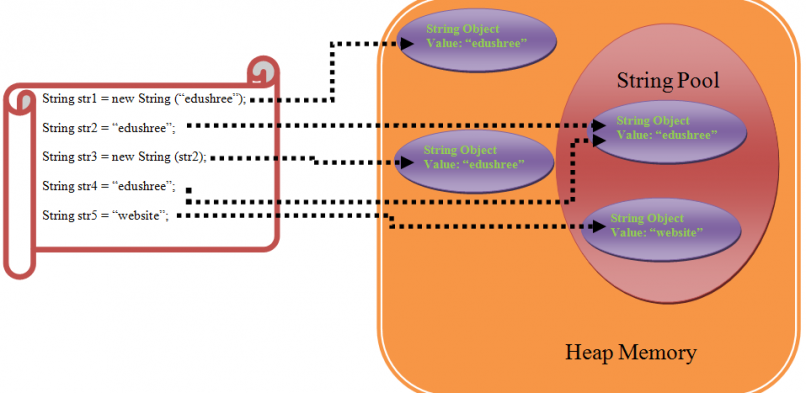
\includegraphics[scale=0.4]{imagenes/pool.png}
\caption{Objetos String}
\end{figure}
\end{frame}


\begin{frame}
\frametitle{Longitud, contenido y concatenación en String}
\begin{figure}
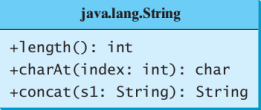
\includegraphics[scale=0.7]{imagenes/longitud.png}
\end{figure}
\pause
\begin{enumerate}[<+->]
\item Devuelve el numero de carácteres en el string.
\item Devuelve el carácter del string en una posición determinada.
\item Devuelve un nuevo string que contatena al string con \emph{s1}
\item La concatenación de cadenas se puede hacer también con el operador \alert{+}
\end{enumerate}
\pause
\begin{figure}
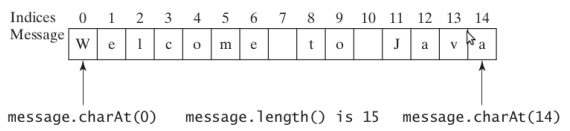
\includegraphics[scale=0.7]{imagenes/art.png}
\end{figure}
\end{frame}

\begin{frame}
\frametitle{Subcadenas}
\begin{figure}
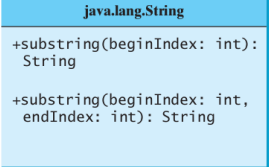
\includegraphics[scale=0.7]{imagenes/substring1.png}
\end{figure}
\pause
\begin{enumerate}[<+->]
\item Devuelve una subcadena del string que empieza en el índice indicado y finaliza al final de la cadena.
\item Devuelve una subcadena del string que comienza en indice especificado como \emph{beginIndex} y acaba en el caracter con índice \emph{endIndex – 1}.
\end{enumerate}
\pause
\begin{figure}
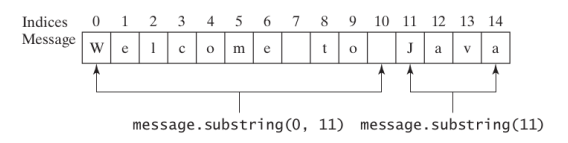
\includegraphics[scale=0.5]{imagenes/substring2.png}
\end{figure}
\end{frame}

\begin{frame}
\frametitle{Convertir, Reemplazar, and Cortar Strings} 
\begin{multicols}{2}
\begin{figure}
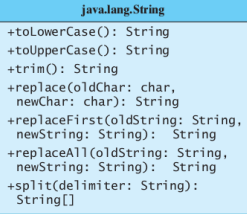
\includegraphics[scale=0.55]{imagenes/split.png} 
\caption{UML de la clase String}
\end{figure} 
\begin{scriptsize}
\begin{enumerate}[<+-| alert@+>]
      \item Devuelve un nuevo string con todos los caracters convertido a minúscula.
      \item Devuelve un nuevo string con todos los caracters convertido a mayúscula.
      \item Devuelve un nuevo string con los caracteres blancos eliminados del principio y final.
     \item Devuelve un nuevo string que reemplaza todas las coincidencias con los nuevos caracteres
      \item Devuelve un nuevo string que reemplaza la primera coincidencia del substring  con el nuevo substring
      \item Devuelve un nuevo string que reemplaza todas las coincidencias del substring  con el nuevo substring
      \item Devuelve un array de strings con los substrings resultantes de cortar el string con un delimitador
            \end{enumerate}
\end{scriptsize}
\end{multicols}
\pause
\end{frame}


\begin{frame}[fragile]
    \frametitle{Ejemplo}
\begin{footnotesize}
\begin{block}{REPLACE,REPLACEALL, TOLOWERCASE Y TOUPPERCASE}
\begin{verbatim}
"Welcome".toLowerCase() devuelve un nuevo string, welcome.
"Welcome".toUpperCase() devuelve un nuevo string, WELCOME.
" Welcome ".trim() devuelve un nuevo string, Welcome.
"Welcome".replace('e', 'A') devuelve un nuevo string, WAlcomA.
"Welcome".replaceFirst("e", "AB") devuelve un nuevo string, WABlcome.
"Welcome".replace("e", "AB") devuelve un nuevo string, WABlcomAB.
"Welcome".replace("el", "AB") devuelve un nuevo string, WABcome.
\end{verbatim} 
\end{block}
\pause
\begin{block}{SPLIT}
\begin{verbatim}
String[] tokens = "Java#HTML#Perl".split("#", 0);
for (int i = 0; i < tokens.length; i++)
System.out.print(tokens[i] + " ");
/* Display Java HTML Per*/
\end{verbatim}
\end{block}
\end{footnotesize}
\end{frame}


\begin{frame}[fragile]
    \frametitle{Expresiones regulares}
    \begin{itemize}[<+->]
    \item A menudo se llaman \emph{regex}
    \item Es una secuencia de caracteres que forma un patrón de búsqueda
    \item Principalmente utilizada para la búsqueda de patrones de cadenas de caracteres u operaciones de sustituciones.
    \item Por ejemplo, el grupo formado por las cadenas Handel, Händel y Haendel
    \item Se describe mediante el patrón ''H(a$|$ä$|$ae)ndel''
    \item Se suelen usar cuantificadores como +, ? y *
    \item El signo más indica que el carácter que le precede debe aparecer al menos una vez. Por ejemplo, "ho+la" describe el conjunto infinito hola, hoola, hooola, hoooola, \dots
    \item El signo de interrogación indica que el carácter que le precede puede aparecer como mucho una vez. Por ejemplo, ''ob?scuro'' se corresponde con oscuro y obscuro.
    \item El asterisco indica que el carácter que le precede puede aparecer cero, una, o más veces. Por ejemplo, "0*42" se corresponde con 42, 042, 0042, 00042, \dots
    \end{itemize}

\end{frame}

\begin{frame}
    \frametitle{matches(regex)}
    \framesubtitle{Todas estas sentencias se evalúan como \alert{true}}
\begin{itemize}[<+-| alert@+>]
\item ''Java''.matches(''Java'');
\item ''Java''.equals(''Java'');.
\item ''Java is fun".matches(''Java.*'' );
\item ''Java is powerful''.matches(''Java.*'' );
\end{itemize}
\pause
\end{frame}

\begin{frame}[fragile]
\frametitle{replaceAll(regex) y split(regex)}
\begin{verbatim}
String s = "a+b$#c".replaceAll("[$+#]", "NNN");
System.out.println(s);
/*muestra aNNNbNNNNNNc*/
\end{verbatim}
\pause
\begin{verbatim}
String[] tokens = "Java,C?C#,C++".split("[.,:;?]");
for (int i = 0; i < tokens.length;
/* muestra Java, C, C# y C++  */
\end{verbatim}
\pause
¿Cómo funciona?
\end{frame}

\begin{frame}[fragile]
\frametitle{Buscando un carácter o substring en un String}
\framesubtitle{indexOf y lastIndexOf}
\begin{scriptsize}
\begin{verbatim}
"Welcome to Java".indexOf('W') devuelve 0.
"Welcome to Java".indexOf('o') devuelve 4.
"Welcome to Java".indexOf('o', 5) devuelve 9.
"Welcome to Java".indexOf("come") devuelve 3.
"Welcome to Java".indexOf("Java", 5) devuelve 11.
"Welcome to Java".indexOf("java", 5) devuelve -1.
"Welcome to Java".lastIndexOf('W') devuelve 0.
"Welcome to Java".lastIndexOf('o') devuelve 9.
"Welcome to Java".lastIndexOf('o', 5) devuelve 4.
"Welcome to Java".lastIndexOf("come") devuelve 3.
"Welcome to Java".lastIndexOf("Java", 5) devuelve -1.
"Welcome to Java".lastIndexOf("Java") devuelve 11.
\end{verbatim}
\pause
\begin{itemize}[<+->]
\item ¿Cómo funciona \alert{indexOf} y \alert{lastIndexOf}?
\item Devuelve \alert{-1} si no hay coincidencia.
\item \alert{indexOf(s:String)} devuelve el índice de la primera ocurrencia.
\item \alert{indexOf(s:String,fromIndex)} devuelve el índice de la primera ocurrencia despues de fromIndex.
\item \alert{lastIndexOf(s:String)} devuelve el índice de la última ocurrencia.
\item \alert{lastIndexOf(s:String,fromIndex)} devuelve el índice de la primera ocurrencia antes de fromIndex.
\end{itemize}
\end{scriptsize}
\pause
\end{frame}


\begin{frame}
\frametitle{Conversión entre String y Arrays}
\framesubtitle{Y viceversa}
\begin{block}{De String a Array}
\begin{itemize}[<+-| alert@+>]
\item char[ ] chars = ''Java''.toCharArray();
\end{itemize}
\end{block}
\pause
\begin{block}{De Array a String }
\begin{itemize}[<+-| alert@+>]
\item String str = new String(new char[ ]\{'J', 'a', 'v', 'a'\});
\end{itemize}
\end{block}
\pause
\end{frame}

\section{Clase Character}
\begin{frame}
\frametitle{Clase Character} 
\begin{multicols}{2}
\begin{figure}
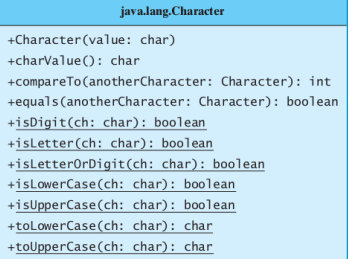
\includegraphics[scale=0.55]{imagenes/char.png} 
\caption{UML de la clase String}
\end{figure} 
\begin{scriptsize}
\begin{enumerate}[<+-| alert@+>]
      \item Constructor de un objeto de la clase Character con el valor \emph{char}.
      \item Devuelve el valor del caracter del objeto.
      \item Compara dos caracteres. 
     \item Devuelve \emph{true} si los dos caracteres son iguales.
      \item Devuelve true si el caracter es una letra.
      \item Devuelve true si el caracter es una letra o un dígito.
      \item Devuelve true si el caracter es minúscula.
      \item Devuelve true si el caracter es mayúscula.
      \item Devuelve el caracter en minúscula.
      \item Devuelve el caracter en mayúscula.
      \end{enumerate}
\end{scriptsize}
\end{multicols}
\pause
\end{frame}

\section{Clase StringBuilder/StringBuffer}

\begin{frame}
\frametitle{La clase StringBuilder/StringBuffer}
\begin{footnotesize}
\begin{itemize}[<+->]
\item Es una alternativa a la clase String.
\item Puede ser usada donde exista un String.
\item Es mas flexible que la clase String.
\item \emph{String} es un objeto inmutable y \emph{StringBuilder} no lo es.
\item Los método de \emph{StringBuilder} son mas eficientes
\item Se puede añadir, insertar, \dots en un \emph{StringBuilder} o un \emph{StringBuffer}
\item Mientrás que el valor del String siempre es fijo.
\end{itemize}
\end{footnotesize}
\pause
\begin{block}{Constructores}
\begin{figure}
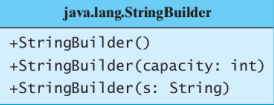
\includegraphics[scale=0.7]{imagenes/sb1.png}
\end{figure}
\end{block}
\pause
\begin{footnotesize}
\begin{itemize}[<+->]
\item Construye un string builder vacío
\item Idem pero con una capacidad dada.
\item Idem pero con un string.
\end{itemize}
\end{footnotesize}
\end{frame}

\begin{frame}
\frametitle{Capacidad y tamaño}
\begin{figure}
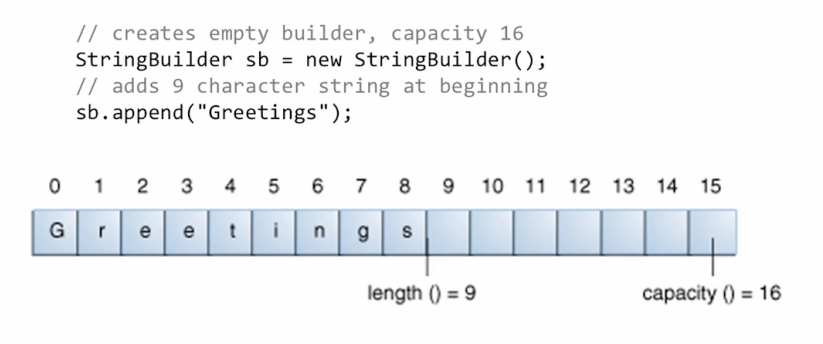
\includegraphics[scale=0.5]{imagenes/capacidad.png}
\end{figure}
\end{frame}



\begin{frame}
\frametitle{Clase StringBuilder/StringBuffer} 
%me quedo aquí
\begin{multicols}{2}
\begin{figure}
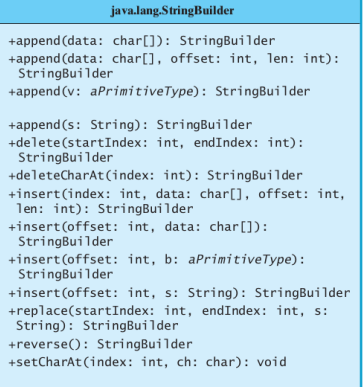
\includegraphics[scale=0.55]{imagenes/sb2.png} 
\caption{UML de la clase String Builder}
\end{figure} 
\begin{tiny}
\begin{enumerate}[<+-| alert@+>]
      \item Añade un char array dentro del string builder.
      \item Añade un subarray de char dentro del string builder.
      \item Añade un tipo primitivo como string dentro del string builder. 
     \item Añade un string al string builder.
      \item Borra caracteres desde startIndex a endIndex-1.
      \item Inserta un subarray de char al string builder al índice especificado.
      \item Inserta subrray char al string builder en la posición offset.
      \item Inserta un valor primitivo convertido a string dentro del string builder en la posición offset.
      \item Inserta un string dentro del string builder a la posición offset.
      \item Reemplazas los caracteres en el string builder desde startIndex
a endIndex-1 con el  especificado string.
	\item Invierte los caracteres en el string builder.
	\item Fija un nuevo caracter en el índice especificado en el string builder.
      \end{enumerate}
\end{tiny}
\end{multicols}
\pause
\end{frame}

\begin{frame}[fragile]
\frametitle{Ejemplo de string builder}
\begin{footnotesize}
\begin{verbatim}
StringBuilder stringBuilder = new StringBuilder();
stringBuilder.append("Welcome");
stringBuilder.append(' ');
stringBuilder.append("to");
stringBuilder.append(' ');
stringBuilder.append("Java");
//stringBuilder contine "Welcome to Java"
stringBuilder.insert(11, "HTML and ");
//El nuevo stringBuilder es "Welcome to HTML and Java".
stringBuilder.delete(8, 11) 
//cambia el string builder a "Welcome Java."
stringBuilder.deleteCharAt(8) cambia a "Welcome o Java".
stringBuilder.reverse() cambia a "avaJ o emocleW."
stringBuilder.reverse(); stringBuilder.insert(8, "t");
//El nuevo stringBuilder es "Welcome to Java".
stringBuilder.replace(11, 15, "HTML"); cambia "Welcome to HTML."
stringBuilder.setCharAt(0, 'w'); cambia a "welcome to Java."
\end{verbatim}
\end{footnotesize}
\end{frame}

\begin{frame}
\frametitle{String Builder} 
\begin{multicols}{2}
\begin{figure}
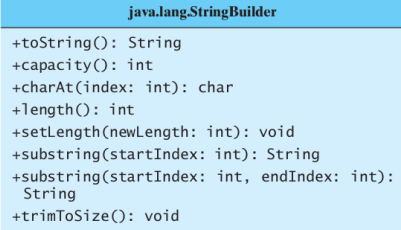
\includegraphics[scale=0.55]{imagenes/sb3.png} 
\caption{UML de la clase String Builder}
\end{figure} 
\begin{scriptsize}
\begin{enumerate}[<+-| alert@+>]
      \item Devuelve un string desde the string builder.
      \item Devuelve la capacidad del string builder.
      \item Devuelve el caracter del índice especifcado .
      \item Fija una nueva capacidad para el string buider.
      \item Devuelve un substring comezando en startIndex.
      \item Devuelve un substring desde startIndex a endIndex-1.
      \item Reduce el almacenamientos usado por el string builder.
      \end{enumerate}
\end{scriptsize}
\end{multicols}
\pause
\end{frame}


\begin{frame}
\frametitle{Preguntas} 
\begin{figure}

\includegraphics[scale=0.9]{imagenes/dudas.png} 
\end{figure} 
\end{frame}

\end{document}

